\section{Алгоритмы решения граничных обратных задач}\label{sec:ch4/sec3}

%dvmg368

\subsection{Градиентный спуск и модификации}
\label{subsec:ch4/sec3/grad}


Приведем здесь для удобства классические алгоритмы оптимизации методом градиентного спуска,
которые далее используются при разработке конкретных алгоритмов решения обратных задач.
\textit{Градиентный спуск} -- это способ минимизации целевой функции
$f(\mathbf{x}), \mathbf{x} \in X$, путем обновления параметров
в направлении, противоположном градиенту целевой функции
$\nabla f(\mathbf{x})$.
Скорость обучения $\eta$ определяет размер шагов, которые мы делаем,
чтобы достичь (локального) минимума.
Иными словами, мы следуем направлению наклона поверхности,
созданной целевой функцией, вниз до тех пор,
пока не достигнем локального минимума.

Известны различные способы модификации градиентного спуска.
Перечислим некоторые из них.

\textbf{Градиентный спуск с проекцией}

Метод градиентного спуска широко используется для минимизации дифференцируемой
функции $f(\mathbf{x})$, итеративно двигаясь в направлении наибольшего убывания.
Алгоритм осуществляется путем обновления параметров
$\mathbf{x} \in \mathbb{X}$, где $\mathbb{X}$ некоторое гильбертово пространство,
в направлении, противоположном
градиенту функции $\nabla f(\mathbf{x})$ с величиной шага
(скорость обучения) $\eta$.
Этот простой, но мощный алгоритм оптимизации используется во
множестве приложений, таких как машинное обучение, компьютерное
зрение и обработка сигналов.
В некоторых случаях задача оптимизации
имеет дополнительные ограничения, которые могут быть включены в
алгоритм градиентного спуска с использованием проекции.
Представим краткий обзор метода градиентного спуска с проекцией.


Цель алгоритма градиентного спуска - минимизировать функцию
$f(\mathbf{x})$, итеративно обновляя параметры следующим образом:
\[ \mathbf{x}_{k+1} = x_k - \eta \nabla f(\mathbf{x}_k), \]
где $\mathbf{x}_k$ -- вектор параметров на итерации $k$,
$\eta$ -- величина шага, и $\nabla f(\mathbf{x}_k)$ -- градиент
функции на итерации $k$.
Когда задача оптимизации включает ограничения, алгоритм
градиентного спуска должен быть изменен, чтобы учесть эти ограничения.
Один из распространенных подходов состоит в использовании проекции
на множество ограничений.


Пусть $\mathcal{C}$ -- множество ограничений.
Алгоритм градиентного спуска с проекцией
можно описать следующим образом:
\[ x_{k+1} = \mathcal{P}_{\mathcal{C}}(x_k - \eta \nabla f(x_k)), \]
где $\mathcal{P}_{\mathcal{C}}(\cdot)$ -- оператор проекции
на множество ограничений $\mathcal{C}$.
Проекция обеспечивает сохранение обновленного
вектора параметров $\mathbf{x}_{k+1}$ в пределах множества
ограничений, таким образом, удовлетворяя ограничениям задачи.

\textbf{Оператор проекции}

Оператор проекции $\mathcal{P}_{\mathcal{C}}(\cdot)$
проецирует заданную точку на множество ограничений $\mathcal{C}$.
Проекция точки $\mathbf{y}$ на множество $\mathcal{C}$ определяется как
\[
    \mathcal{P}_{\mathcal{C}}(y) =
    \arg \min_{x \in \mathcal{C}} \|y - x\|^2,
\]
где $\|\cdot\|$ обозначает евклидову норму.
Оператор проекции находит точку в множестве ограничений
$\mathcal{C}$, которая ближе всего к заданной точке $\mathbf{y}$.

\textbf{Примеры множеств ограничений}

Множество ограничений может иметь различные формы
в зависимости от задачи оптимизации.
Некоторые распространенные множества ограничений включают:
\begin{itemize}
    \item \textbf{Ограничения-коробки:} Множество ограничений представляет
    собой коробку, определенную как
    $\mathcal{C} = \{\mathbf{x} \in \mathbb{R}^n , | , a_i
    \leq x_i \leq b_i, , i=1,\dots,n\}$.
    В этом случае оператор проекции можно вычислить поэлементно:
    \[
        (\mathcal{P}_{\mathcal{C}}(y))_i =
        \min(\max(y_i, a_i), b_i), \quad i=1,\dots,n.
    \]

    \item \textbf{Ограничения-шары:} Множество ограничений представляет
    собой закрытый шар с радиусом $r$ и центром $\mathbf{c}$,
    определенный как $\mathcal{C} = \{\mathbf{x} \in \mathbb{R}^n , | ,
    \|\mathbf{x} - \mathbf{c}\| \leq r\}$.
    Оператор проекции для этого множества ограничений:
    \[
        \mathcal{P}_{\mathcal{C}}(y) = c
        + \min\left(1, \frac{r}{\|y-c\|}\right)(y-c).
    \]
    \item \textbf{Ограничения-симплексы:} Множество ограничений
    представляет собой симплекс, определенный как
    $\mathcal{C} = \{\mathbf{x} \in \mathbb{R}^n ,
    | , \mathbf{x} \geq \mathbf{0}, , \sum_{i=1}^n x_i = 1\}$.
    Оператор проекции для этого множества ограничений включает
    более сложный алгоритм, такой как тот,
    который представлен, например~\cite{Duchi2011}.
\end{itemize}

\subsection{Алгоритм нахождения квазирешения обратной задачи}
\label{subsec:ch4/sec3/boundary}

Задача нахождения квазирешения обратной
задачи (см.~\ref{subsec:ch2/sec1/subsec1})
\begin{equation}
    \label{eq:4_3:initial}
    \begin{aligned}
        - a \Delta \theta + b \kappa_a(\theta ^ 3 | \theta | - \varphi) = 0,  \\
        - \alpha \Delta \varphi + \kappa_a (\varphi - \theta ^3 | \theta |) = 0.
    \end{aligned}
\end{equation}
\begin{equation}
    \label{eq:4_3:initial-boundary}
    \begin{aligned}
        \Gamma &: \; a \partial_n \theta + \beta (\theta - \theta _b) = 0, \\
        \Gamma_0 \cup \Gamma_2 &: \; \alpha \partial_n \varphi
        + \gamma(\varphi - \theta_b ^4 ) = 0, \\
        \Gamma_1 &: \; \alpha \partial_n \varphi + u(\varphi - \theta_b ^4 ) = 0,
    \end{aligned}
\end{equation}
где предполагается, что неизвестная функция $u$ удовлетворяет неравенствам:
\begin{equation}
    \label{eq:4_3:control_bounds}
    0 < u_1 \leq u \leq u_2,
\end{equation}
а также условию $\theta = \theta_0$ на $\Gamma_2$,
заключается в минимизации функционала~\eqref{eq:2_1:quality}
\begin{equation}
    \label{eq:4_3:quality}
    J(\theta) = \frac{1}{2} \int_{\Gamma_2} (\theta - \theta_0)^2 d\Gamma
\end{equation}
на решениях начально-краевой задачи~\eqref{eq:4_3:initial}--\eqref{eq:4_3:control_bounds}.

Пусть функционал $J(\theta)$ удовлетворяет условиям,
указанным в~\autoref{subsec:ch2/sec1/subsec3}.
Для удобства введём переобозначение
$\hat{J}(u)\coloneqq J(\theta(u)), \hat{J}:L^2(\Gamma_1) \to \mathbb{R}$.
Здесь $\theta(u)$ -- температурное поле
задачи~\eqref{eq:2_1:initial}--\eqref{eq:2_1:initial-boundary}
отвечающее управлению $u \in L^2(\Gamma_1)$.

Согласно формуле~\eqref{eq:2_1:theorem_2_eq3}
градиент функционала $\hat{J}(u)$ имеет вид
\[
    \hat{J}'(u)= (\varphi(u) -\theta_b^4)p_2,
\]
где $\varphi(u)$ есть интенсивность излучения,
$p_2$ -- соответствующая переменная сопряжённой
системы~\eqref{eq:2_1:theorem_2_eq1}--\eqref{eq:2_1:theorem_2_eq3}
\begin{gather*}
    A_1 p_1 + 4 |\hat{\theta}|^3 \kappa_a(b p_1 - p_2) = f_c,
    \;\; (f_c,v) = - \int_{\Gamma_2} (\hat{\theta} - \theta_0) v d\Gamma, \\
    A_2 p_2 + \kappa_a (p_2-b p_1) = g_c(p_2, \hat{u}),
    \;(g_c(p_2, \hat{u}), v) = -\int_{\Gamma_1} \hat{u} p_2 v d\Gamma, \\
    \int_{\Gamma_1} p_2 (\hat{\varphi} - \theta_b^4)(u-w) d\Gamma
    \leq 0 \quad \forall w \in U_{ad}.
\end{gather*}


Предлагаемый алгоритм решения выглядит следующим образом:

%\begin{algorithm}[H]
%    \caption{Алгоритм градиентного спуска с проекцией}
%    \begin{algorithmic}[1]
%        \State Выбираем значение градиентного шага $\lambda$,
%        \State Выбираем количество итераций $N$,
%        \State Выбираем произвольное $u_0 \in U_{ad}$,
%        \For{$k \gets 0,1,2,...,N$}
%            :
%            \State Для полученного $u_k$ расчитываем состояние $y_k = \{\theta_k, \varphi_k\}$ из  (\ref{weak_operational}).
%            \State Расчитываем значение функционала качества $J(\theta_k)$ из (\ref{quality}).
%            \State Расчитываем сопряжённое состояние $p_k=\{p_{1k},p_{2k}\}$ из уравнений \eqref{eq:2_1:theorem_2_eq1}--\eqref{eq:2_1:theorem_2_eq2}, где $ \hat{\theta} := \theta_k, \hat{u}=u_k$.
%            \State Пересчитываем управление $u_{k+1} = P_{ad}\left[ u_k - \lambda (\varphi_k - \theta_b^4)p_{2k} \right]$.
%        \EndFor
%    \end{algorithmic}
%\end{algorithm}

\textbf{Алгоритм градиентного спуска с проекцией}

1.\ Выбор значения шага градиента $\lambda$.

2.\ Выбор числа итераций $N$.

3.\ Выбор начального приближения для управления $u_0 \in U_{ad}$.

4.\ для $k \leftarrow 0,1,2, \ldots, N$ выполнить:

\hspace{1cm} a.\ Для заданного $u_{k}$, вычислить состояние $y_k = \{\theta_k, \varphi_k\}$
системы~\eqref{eq:2_1:weakOperational}.

\hspace{1cm} b.\ Вычислить значение функционала качества
$J(\theta_k)$ из уравнения~\eqref{eq:2_1:quality}.

\hspace{1cm} c.\ Рассчитать сопряжённое состояние $p_k=\{p_{1k},p_{2k}\}$ из
уравнений~\eqref{eq:2_1:theorem_2_eq1}--\eqref{eq:2_1:theorem_2_eq2},
где $ \hat{\theta} \coloneqq \theta_k, \hat{u}=u_k$.

\hspace{1cm} d.\  Пересчитать управление
$u_{k+1} = P_{ad}\left[ u_k - \lambda (\varphi_k - \theta_b^4)p_{2k} \right]$.


Значение параметра $\lambda$ выбирается согласованным со значением
градиента $J^{\prime}\left(u_{k}\right)=$ $=\left(\varphi_{k}-\theta_{b}^{4}\right) p_{2k}$
таким образом, чтобы значение $\lambda\left(\varphi_{k}-\theta_{b}^{4}\right) p_{2k}$
определяло значимую поправку для $u_{k}$.
В экспериментах, приведённых ниже, значение параметра $\lambda=20$.

Количество итераций $N$ выбирается достаточным для выполнения условия
$J\left(\theta_{N-1}\right)-J\left(\theta_{N}\right)<10^{-15}$.
Эксперименты показывают хорошее восстановление функции $u$ при $N>10^{5}$.

Оператор проекции $P_{ad} : U \to U_{ad}$ определён следующим образом:
\[
    P_{ad}[v] =
    \begin{cases}
        u_1, & \text{если } v \le u_1 \\
        v, & \text{если } u_1 < v < u_2 \\
        u_2, & \text{если } v \ge u_2.
    \end{cases}
\]

\subsection{Примеры численного моделирования для двумерного случая}
\label{subsec:ch4/sec3/numeric-samples}

Положим $\Omega = \{(x,y), 0 \leq x,y \leq 1\}$, $l = 1$ см.
Граница $\partial\Omega$ состоит из участков:
\[
    \begin{aligned}
        \Gamma_0 & = \{x=\{0,1\}, y \in [0,1]\} \\
        \Gamma_1 & = \{x\in [0,1], y=0\}
        - \text{участок с неизвестными отражающими свойствами}, \\
        \Gamma_2 & = \{x \in [0,1], y=1\} - \text{участок наблюдения}.
    \end{aligned}
\]

Будем также далее считать, что $a = 0.006[\text{см}^2/\text{c}]$,
$b=0.025[\text{см}/\text{с}]$, $\beta = 0.00005[\text{см}/\text{с}]$,
$\kappa=1[\text{см}^{-1}]$, $\kappa_s = 0$, $A = 0$, $\gamma = 0.3$.
Указанные параметры соответствуют стеклу~\cite{Grenkin2016a}.
Температуру на границе $\Omega$ положим равной $\theta_b = (x^2+y^2)/3$.

При указанных параметрах для первого эксперимента выберем следующее тестовое
значение функции $u$ (рис.~\ref{fig:4_3:control}а):
\begin{equation}
    \label{eq:4_3:equation}
    u(x)=
    \begin{cases}
        0.01, & \text{если } x \le 0.5, \\
        0.5, & \text{если } x > 0.5,
    \end{cases}
\end{equation}
и для второго эксперимента (рис.~\ref{fig:4_3:control}б):
\begin{equation}
    \label{eq:4_3:test_function_1}
    u(x)=0.49x+0.01.
\end{equation}

Вычислим решение прямой
задачи~\eqref{eq:2_1:initial}--\eqref{eq:2_1:initial-boundary}
для этих случаев.
Полученное температурное поле на участке наблюдения
$\Gamma_2$ выберем в качестве $\theta_0$.
Далее, применяя предложенный алгоритм, находим квазирешение обратной
задачи~\eqref{eq:2_1:initial}--\eqref{eq:2_1:theta_gamma}.
Эффективность алгоритма, а также значение $u_0$ в первом и
втором случаях иллюстрируются на рисунке~\ref{fig:4_3:control}.
На рисунке~\ref{fig:4_3:cost} показана динамика функционала качества по итерациям.
\begin{figure}[h!t]
    \begin{minipage}[b][][b]{0.49\linewidth}
        \centering
        \includegraphics[width=1\linewidth]{dvmg368/3} \\ а) Первый эксперимент
    \end{minipage}
    \hfill
    \begin{minipage}[b][][b]{0.49\linewidth}
        \centering
        \includegraphics[width=1\linewidth]{dvmg368/4} \\ б) Второй эксперимент
    \end{minipage}
    \caption{Значение функционала качества}
    \label{fig:4_3:cost}
\end{figure}

\begin{remark}
    В предложенных примерах потребовалось
    $2 \cdot 10^6$ итераций для нахождения квазирешения $u$.
    В то же время температурное поле на участке наблюдения
    $\Gamma_2$ становится близким к $\theta_0$ уже на $10^2$ итерации.
    Также наблюдается существенное падение скорости уменьшения функционала
    качества с каждой итерацией после того, как среднее значение найденной
    функции контроля становится близко к тестовой функции.
\end{remark}

\begin{figure}[h!t]
    \begin{minipage}[b][][b]{0.49\linewidth}
        \centering
        \includegraphics[width=1\linewidth]{dvmg368/1} \\ а) Первый эксперимент
    \end{minipage}
    \hfill
    \begin{minipage}[b][][b]{0.49\linewidth}
        \centering
        \includegraphics[width=1\linewidth]{dvmg368/2} \\ б) Второй эксперимент
    \end{minipage}
    \caption{Тестовая функция $u$, начальная $u_0$, найденная функция $u_{end}$.}
    \label{fig:4_3:control}
\end{figure}

\subsection{Алгоритм решения задачи оптимального управления для квазистационарной модели}
\label{subsec:ch4/sec3/quasistationary}
%paper03
Задача оптимального управления, поставленная в разделе~\ref{sec:ch2/sec3}
для квазистационарной модели имеет вид:
\begin{equation*}
    J_{\lambda}(\theta, u)=\frac{1}{2} \int_{0}^{T}
    \int_{\Gamma}\left(\theta-\theta_{b}\right)^{2} d \Gamma d t+\frac{\lambda}{2}
    \int_{0}^{T} \int_{\Gamma} u^{2} d \Gamma d t \rightarrow \inf
\end{equation*}
при ограничениях
\begin{equation}
    \label{eq:4_3:1}
    \begin{split}
        & \frac{\partial \theta}{\partial t} - a \Delta \theta
        + b \kappa_{a} \left(|\theta| \theta^{3}-\varphi\right) = 0,\\
        & - \alpha \Delta \varphi
        + \kappa_{a} \left(\varphi-|\theta| \theta^{3}\right) = 0,
        \quad x \in \Omega, \quad 0 < t < T;
    \end{split}
\end{equation}
\begin{align}
    a \left(\partial_{n} \theta+\theta\right)=r,
    & \quad \alpha\left(\partial_{n} \varphi
    + \varphi\right) = u \text { на } \Gamma;  \label{eq:4_3:2}\\
    & \left.\theta\right|_{t=0} = \theta_{0}. \label{eq:4_3:3}
\end{align}
Напомним, что эта задача аппроксимирует задачу с данными типа Коши для температуры.


Приведем алгоритм решения задачи управления.
Пусть
\[
    \widetilde{J}_{\lambda}(u)=J_{\lambda}(\theta(u), u),
\]
где $\theta(u)$ — компонента решения
задачи~\eqref{eq:2_3:1}--\eqref{eq:2_3:2},
соответствующая управлению $u \in U$.
Согласно~\eqref{eq:2_3:15} градиент функционала
$\widetilde{J}_{\lambda}(u)$ определяется
следующим образом: $\widetilde{J}_{\lambda}^{\prime}(u) = \lambda u-p_{2}$.
Здесь $p_{2}$ — соответствующая компонента сопряженного
состояния системы~\eqref{eq:2_3:15}
\begin{gather*}
    -p_{1}^{\prime}+a A p_{1}+4|\widehat{\theta}|^{3} \kappa_{a}\left(b p_{1}
    -p_{2}\right)=B\left(\theta_{b}-\widehat{\theta}\right), \\
    p_{1}(T)=0,\; \alpha A p_{2}+\kappa_{a}\left(p_{2}-b p_{1}\right)=0,
\end{gather*}
где $\widehat{\theta}\coloneqq\theta(u)$.
Предлагаемый алгоритм для решения задачи оптимального управления
состоит из следующих шагов:

\textbf{Алгоритм градиентного спуска}

1.\ Выбор значения шага градиента $\varepsilon$,

2.\ Выбор числа итераций $N$,

3.\ Выбор начального приближения для управления $u_{0} \in U$,

4.\ для $k \leftarrow 0,1,2, \ldots, N$ выполнить:

\hspace{1cm} a.\ Для заданного $u_{k}$, вычислить состояние
$y_{k}=\left\{\theta_{k}, \varphi_{k}\right\}$, решение
задачи~\eqref{eq:2_3:1}--\eqref{eq:2_3:3}.

\hspace{1cm} b.\ Вычислить значение функционала качества
$J_{\lambda}\left(\theta_{k}, u_{k}\right)$.

\hspace{1cm} c.\ Из уравнений~\eqref{eq:2_3:15}, вычислить сопряженное
состояние $p_{k}=\left\{p_{1 k}, p_{2 k}\right\}$,
где $\widehat{\theta} \coloneqq \theta_{k}, \widehat{u} \coloneqq u_{k}$.

\hspace{1cm} d.\ Пересчитать управление
$u_{k+1}=u_{k}-\varepsilon\left(\lambda u_{k}-p_{2}\right)$.

Параметр $\varepsilon$ выбирается эмпирически таким образом, чтобы
значение $\varepsilon\left(\lambda u_{k}-p_{2}\right)$ являлось
существенной корректировкой для $u_{k+1}$.
Число итераций $N$ выбирается достаточным для
удовлетворения условия $J_{\lambda}\left(\theta_{k}, u_{k}\right)
-J_{\lambda}\left(\theta_{k+1}, u_{k+1}\right)<\delta$, где $\delta>0$
определяет точность вычислений.

Рассмотренный ниже пример иллюстрирует работу предложенного
алгоритма для малых, что важно, значений параметра регуляризации
$\lambda \leq 10^{-12}$.


Заметим, что для численного решения прямой задачи с заданным управлением
был использован метод простой итерации для линеаризации задачи и ее решения
с помощью метода конечных элементов.
Для численного моделирования мы использовали солвер FEniCS~\cite{fenics, dolfin}.
Сравним работу предложенного
алгоритма с результатами статьи~\cite{Chebotarev2019Problem}.
Задача рассматривается в области $\Omega \times(-L, L)$,
где $\Omega=$ $\left\{x=\left(x_{1}, x_{2}\right): 0<x_{1,2}<d\right\}$
и при большом $L$ сводится к двумерной задаче для вычислительной
области $\Omega$.

Для задачи были выбраны следующие значения параметров:
$d=1(\text{м}), a=0.9210^{-4}(\text{м}^{2} / \text{с}),
b=0.19(\text{м} / \text{с})$, $\alpha=0.0333(\text{м}),
\kappa_{a}=1\left(\text{м}^{-1}\right)$.
Параметры соответствуют воздуху при нормальном атмосферном давлении
и температуре $400^{\circ} \text{C}$.
Функции $\theta_{b}, q_{b}$ для граничного условия~\eqref{eq:2_3:5}
задаются следующим образом: $\theta_{b}=\left.\widehat{\theta}\right|_{\Gamma},
q_{b}=\left.\partial_{n} \widehat{\theta}\right|_{\Gamma}$,
где $\widehat{\theta}=$ $\left(x_{1}-0.5\right)^{2}-0.5 x_{2}+0.75$.

Приближенное решение задачи~\eqref{eq:2_3:16},~\eqref{eq:2_3:17}
с данными Коши, представленными в~\cite{Chebotarev2019Problem}
(рисунок~\ref{fig:4_3:1}а), было получено путем решения параболической задачи
четвертого порядка для температуры.
Решение стабилизировалось через 120 секунд, но
вычисления на каждом временном шаге были
довольно затратными.
\begin{figure}[h!t]
    \begin{minipage}[b][][b]{0.49\linewidth}
        \centering
        \includegraphics[width=1\linewidth]{paper03/1} \\ а) Поле температуры,
        полученное в статье~\cite{Chebotarev2019Problem}
    \end{minipage}
    \hfill
    \begin{minipage}[b][][b]{0.49\linewidth}
        \centering
        \includegraphics[width=1\linewidth]{paper03/2} \\
        б) Поле температуры, полученное предложенным алгоритмом
    \end{minipage}
    \caption{сравнение полученных температурных полей}
    \label{fig:4_3:1}
\end{figure}
На рисунке~\ref{fig:4_3:1}б показано стационарное поле температуры,
полученное с помощью метода, предложенного в данном параграфе.

Представленный пример иллюстрирует, что предложенный
алгоритм успешно находит численное решение
задачи~\eqref{eq:2_3:16},~\eqref{eq:2_3:17} с граничными
условиями типа Коши.

%6_Chebotarev

%6_cheb
%


%Перенос тепла и излучения будет рассматриваться в среде,
%состоящей из четырех частей, которые интерпретируются как кровь,
%стенки вены, около-венозная ткань и оптическое волокно.
%Вычислительная область в цилиндрической системе координат в случае
%угловой симметрии схематически изображена на рисунке~\ref{fig:4_3:3}
%(линейные размеры указаны в миллиметрах).
%
%\begin{figure}[h!t]
%    \centerfloat{\includegraphics[scale=0.35]{6_cheb/1}}
%    \caption{Область вычисления}
%    \label{fig:4_3:3}
%\end{figure}
%%\ref{fig:4_3:3}
%Для нахождения решения начально-краевой
%задачи~\eqref{eq:1_6:1}--\eqref{eq:1_6:3}
%мы дискретизируем временной интервал
%$(0, T), \quad 0=t_{0}<t_{1}<t_{2}<\ldots<t_{N}=T$.
%Для каждого момента времени $t=t_{l}=l \Delta t, l=1,2, \ldots, N$,
%используется итерационный алгоритм для нахождения решения соответствующей
%краевой задачи. $n$-й шаг итерационной процедуры $(n=1,2, \ldots, M)$
%записывается следующим образом:
%\begin{gather}
%    -\operatorname{div}\left(\alpha \nabla \varphi_{n}\right)
%    +\beta\left(\varphi_{n}-\theta_{n-1}^{3}
%    \left|\theta_{n-1}\right|\right)=g, \label{eq:3_1:22}\\
%    \sigma \partial \theta_{n} / \partial t
%    -\operatorname{div}\left(k\left(\theta_{n-1}\right)
%    \nabla \theta_{n}\right)
%    -b\left(\theta_{n-1}^{3}\left|\theta_{n}\right|
%    -\varphi_{n}\right)=f, \quad x \in \Omega, \label{eq:3_1:23}\\
%    k\left(\theta_{n-1}\right) \partial_{n} \theta_{n}
%    +\left.p\left(\theta_{n}-\theta_{b}\right)\right|_{\Gamma}=0,
%    \quad \alpha \partial_{n} \varphi_{n}+\left.\gamma
%    \left(\varphi_{n}-\theta_{b}^{4}\right)\right|_{\Gamma}=0,\label{eq:3_1:24}
%\end{gather}
%где производная по времени в~\eqref{eq:3_1:23}
%аппроксимируется как:
%\[
%    \frac{\partial \theta_{n}}{\partial t} \simeq
%    \frac{
%        \left.\theta_{n}\right|_{t=t_{l}}
%        -\left.\theta_{M}\right|_{t=t_{l-1}}
%    }{\Delta t},
%\]
%и функции $\theta_{n}, \theta_{n-1}, \varphi_{n}$
%в~\eqref{eq:3_1:22}--\eqref{eq:3_1:24} являются приближениями решения,
%соответствующими моменту времени $t=t_{l}$.
%Подстрочный индекс функций
%$\theta_{n}, \theta_{n-1}$ и $\varphi_{n}$ означает номер итерации.
%Для инициализации итерационной процедуры задаем начальное приближение
%температуры для каждого момента времени:
%\begin{equation}
%    \label{eq:3_1:25}
%    \left.\theta_{0}\right|_{t=t_{l}}=
%    \left.\theta_{M}\right|_{t=t_{l-1}},
%    \quad l=1,2, \ldots, N, \left.\quad
%    \theta_{M}\right|_{t=t_{0}}=\theta_{i n}.
%\end{equation}
%
%В уравнениях~\eqref{eq:3_1:22},~\eqref{eq:3_1:23}
%$g=P_{\varphi} \chi / \mathcal{M}_{\varphi},
%f=P{\theta} \chi / \mathcal{M}_{\theta}$,
%где $P{\varphi}$ --  мощность источника, расходуемая на излучение,
%$P_{\theta}$ описывает мощность источника, расходуемую на нагрев
%кончика волокна, $\chi$ -- характеристическая функция части среды,
%в которой расположен кончик волокна, деленная на объем кончика волокна,
%$\mathcal{M}_{\varphi}$ и $\mathcal{M}_{\theta}$ --  нормализующие коэффициенты
%для получения средней интенсивности излучения
%и абсолютной температуры из $\varphi$ и $\theta$.
%
%Для реализации каждого шага итерационного
%алгоритма~\eqref{eq:3_1:22}--\eqref{eq:3_1:25}
%использовался метод конечных элементов с использованием
%программного пакета FreeFEM++\cite{Hecht2012}.
%Оптические и термофизические параметры среды
%взяты из~\cite{van2014optical}.
%Параметры $\theta_{b}$ и $\theta_{i n}$ соответствуют
%температуре $37^{\circ} \text{C}$, а коэффициент $\gamma$ равен 1.
%Во всех расчетах начальное положение кончика оптического волокна
%соответствует $(r, z)=(0,5)$, и его скорость отката составляет
%$2 \text{~мм} / \text{с}$.
%Следуя~\cite{van2014optical, Some_Poluektova2014},
%мы моделируем теплоперенос потоком пузырьков,
%образующихся на горячем кончике волокна, через коэффициент теплопроводности,
%зависящий от температуры, как следующим образом: когда температура
%в определенной точке достигает $95^{\circ}\text{~C}$ и выше,
%коэффициент теплопроводности увеличивается в 200 раз.
%
%Эффективность лазерной абляции можно оценить по поведению
%температурных профилей в различных точках вычислительной области.
%Основные параметры процедуры лазерной абляции -- мощность лазера,
%длина волны излучения, скорость отката оптического волокна и
%соотношение между мощностями лазера, затрачиваемыми на
%излучение и нагрев кончика волокна.
%
%Отметим, что решение задачи~\eqref{eq:1_6:1}--\eqref{eq:1_6:3} зависит от длины
%волны неявным образом, через параметры $\alpha$ и $\beta$,
%описывающие свойства излучения среды (смотрите таблицы значений коэффициента
%поглощения и коэффициента уменьшения рассеяния, определяющие параметры
%$\alpha$ и $\beta$~\cite{van2014optical, Some_Poluektova2014}).
%Как правило, лазерная абляция осуществляется излучением с длиной волны
%от \(810\) до $1950$~нм.
%Достаточно широко используемые диапазоны скорости отката волокна и мощности
%лазерного излучения составляют $1-3\text{~мм}/\text{с}$
%и $5-15$~Вт
%соответственно~\cite{
%    Mathematical_Mordon2006,
%    van2014optical,
%    Some_Poluektova2014}.
%
%
%\begin{figure}[h!t]
%    \centerfloat{\includegraphics[scale=0.33]{6_cheb/2}}
%    \caption{Поведение температуры в точке $(1.5,10)$
%        при мощности лазера $10\text{~Вт}$ и следующих длинах волн:
%        $810\text{~нм}$ (черный), $1064\text{~нм}$ (красный),
%        $1470\text{~нм}$ (зеленый) и $1950\text{~нм}$ (синий).}
%    \label{fig:4_3:4}
%\end{figure}
%
%Рисунок~\ref{fig:4_3:4} показывает поведение температурных профилей в точке $(1.5,10)$ для
%излучения с различными длинами волн: $810 \text{~нм}, 1064 \text{~нм},
%1470 \text{~нм}$ и $1950 \text{~нм}$.
%Мощность источника устанавливается как $\left(P_{\varphi}, P_{\theta}\right)
%=(7 \text{~Вт}, 3 \text{~Вт})$ во всех случаях.
%Как видно из рисунка~\ref{fig:4_3:4}, изменение длины волны излучения оказывает
%значительное влияние на поведение температурного профиля.
%Тем не менее, возможно обеспечить достаточно близкую продолжительность
%кипения (когда температура выше $95^{\circ} \text{C}$) для температурных
%профилей, соответствующих разным длинам волн, изменив мощность
%лазера $P=P_{\varphi}+P_{\theta}$, сохраняя соотношение
%$P_{\varphi} / P_{\theta}$ равным $7 / 3$ (рисунок~\ref{fig:4_3:4}).
%Отметим, что рассчитанная температура в точках перивенозной ткани,
%$(2.5,10)$ и $(3.5,10)$, довольно безопасна (рисунок~\ref{fig:4_3:5}).
%
%Как видно из проведенных экспериментов, использование компьютерного
%моделирования является перспективным способом определения оптимальных
%параметров излучения, обеспечивающих эффективную и безопасную процедуру ВВЛА.
%
%На рисунке~\ref{fig:4_3:4} показаны температурные профили
%в точке $(1.5, 10)$ для мощности лазера
%$10 \text{~Вт}$ и для разных длин волн: $810 \text{~нм}$ (черный),
%$1064 \text{~нм}$ (красный), $1470 \text{~нм}$
%(зеленый) и $1950 \text{~нм}$ (синий).
%
%\begin{figure}[h!t]
%    \centerfloat{\includegraphics[scale=0.33]{6_cheb/3}}
%    \caption{Поведение температуры в точке $(1.5,10)$
%        для следующих длин волн и мощностей лазера:
%        $810 \text{~нм}, P=10 \text{~Вт}$ (черный);
%        $1064 \text{~нм}, P=11 \text{~W}$ (красный);
%        $1470 \text{~нм}, P=7,5 \text{~W}$ (зеленый);
%        $1950 \text{~нм}, P=6 \text{~W}$ (синий).}
%    \label{fig:4_3:5}
%\end{figure}
%На рисунке~\ref{fig:4_3:5} показаны температурные профили в точке $(1.5,10)$ для разных
%длин волн и мощности лазера: $810 \text{~нм}$, $P=10 \text{~Вт}$
%(черный); $1064 \text{~нм}, P=11 \text{~Вт}$ (красный);
%$1470 \text{~нм}, P=7.5 \text{~Вт}$ (зеленый);
%$1950 \text{~нм}, P=6 \text{~Вт}$ (синий).
%
%
%\begin{figure}[h!t]
%    \centerfloat{\includegraphics[scale=0.33]{6_cheb/4}}
%    \caption{Поведение температуры в точках $(1.5,10)$ (сплошная линия),
%        $(2.5,10)$ (пунктирной линией) и $(3,5,10)$ (пунктирной линией с точкой).
%        Длина волны равна $810 \text{~нм},\left(P_{\varphi},
%        P_{\theta}\right)=(7 \text{~W}, 3 \text{~W})$.}
%    \label{fig:4_3:6}
%\end{figure}
%На рисунке~\ref{fig:4_3:6} показаны температурные профили в точках $(1.5,10)$ (сплошной),
%$(2.5,10)$ (пунктирный) и $(3.5,10)$ (точка-тире).
%Длина волны составляет $810 \text{~нм},\left(P_{\varphi},
%P_{\theta}\right)=(7 \text{~Вт}, 3 \text{~Вт})$
%
%
%%Chebotarev_2 nd, Chebotarev_Park_Mesenev_Kovtanyuk_21
%
%\subsection{Метод штрафов для задачи с фазовыми ограничениями}
%\label{subsec:ch4/sec3/subsec5}
%Квазилинейная модель радиационного и диффузионного теплообмена в ограниченной области
%$\Omega \subset \mathbb{R}^{3}$ с границей $\Gamma=\partial \Omega$
%в разделе~\ref{sec:ch3:sec2} представлена в виде начально-краевой задачи
%следующим образом:
%\begin{equation*}
%    \begin{aligned}
%        & \sigma \partial \theta / \partial t-\operatorname{div}(k(\theta) \nabla \theta)-\beta \varphi=u_{1} \chi, \\
%        & -\operatorname{div}(\alpha \nabla \varphi)+\beta \varphi=u_{2} \chi, \quad x \in \Omega, \quad t \in(0, T), \\
%        & \theta=\left.0\right|_{\Gamma}, \quad \alpha \partial_{n}
%        \varphi+\left.2^{-1} \varphi\right|_{\Gamma}=0,\left.\quad \theta\right|_{t=0}=\theta_{0}.
%    \end{aligned}
%\end{equation*}
%Требуется найти неизвестные интенсивности $u_1,\, u_2$ и соответствующие поля $\theta, \, \varphi$
%по условию
%\[
%    J(\theta)=\int_{0}^{T}
%    \int_{G_{1}}\left(\theta-\theta_{d}\right)^{2} d x d t \rightarrow \inf,
%\]
%при ограничениях
%\[
%    u_{1,2} \geq 0, \quad u_{1}+u_{2} \leq P,\left.\quad \theta\right|_{G_{2}} \leq \theta_{*}.
%\]
%
%В разделе~\ref{subsec:ch3/sec2/penalty} показано, что задачу с ограничениями
%на температуру в области $G_2$ можно
%аппроксимировать задачей со штрафом $P_\varepsilon$.
%
%
%Рассмотрим итерационный алгоритм решения задачи оптимального управления
%$P_{\varepsilon}$ для случая, когда параметры управления
%$u_{1}$ и $u_{2}$ не зависят от времени.
%На каждой итерации алгоритма
%решается линейно-квадратичная задача оптимального управления,
%в которой требуется найти минимум функционала
%\begin{equation}
%    \label{eq:3_2:9}
%    \widehat{J}_{\varepsilon}(\theta)=\int_{0}^{T}
%    \int_{G_{1}}\left(\theta-\theta_{d}\right)^{2} dx dt
%    +\frac{1}{\varepsilon} \int_{0}^{T}
%    \int_{G_{*}}\left(\theta-\theta_{*}\right)^{2} dx dt
%    \rightarrow \inf, \quad u\in U_{ad}
%\end{equation}
%с соответствующими ограничениями
%\begin{equation}
%    \label{eq:3_2:10}
%    \begin{gathered}
%        \sigma \partial \theta / \partial t-\operatorname{div}(k(\widehat{\theta})
%        \nabla \theta)=u, \quad x \in \Omega, \quad 0<t<T, \\
%        \left.\theta\right|_{\Gamma}=0, \quad \theta(x, 0)=\theta_{0}.
%    \end{gathered}
%\end{equation}
%Здесь
%\[
%    \begin{gathered}
%        U_{a d}=\left\{u=u_{1} \chi+u_{2} \beta B^{-1} \chi: u_{1,2} \in \mathbb{R},\right.
%        \left.u_{1,2} \geq 0, u_{1}+u_{2} \leq P\right\}, \\
%        G_{*}=\left\{x \in G_{2}: \hat{\theta}(x, t)>\theta_{*}\right\}.
%    \end{gathered}
%\]
%
%Функция $\widehat{\theta}$ описывает поле температуры,
%найденное на предыдущей итерации.
%В качестве зависимости коэффициента теплопроводности от температуры используется
%гладкая аппроксимация кусочно-постоянной функции, рассмотренная
%в~\cite{van2014optical, Some_Poluektova2014, Endovenous_Malskat2014}.
%
%Как легко видеть, задача~\eqref{eq:3_2:9},~\eqref{eq:3_2:10} сводится к
%нахождению минимума квадратичной функции параметров $u_{1}$ и $u_{2}$
%\[
%    \widehat{J}_{\varepsilon}\left(u_{1} \theta_{1}+u_{2} \theta_{2}+\theta_{3}\right) \rightarrow \inf
%\]
%на треугольнике $\left\{u_{1}, u_{2} \in \mathbb{R}:
%u_{1,2} \geq 0, u_{1}+u_{2} \leq P\right\}$.
%Функции $\theta_{1}, \theta_{2}$ и $\theta_{3}$
%вычисляются заранее как решения следующих линейных
%начально-краевых задач для $x \in \Omega, t \in(0, T)$:
%\[
%    \begin{aligned}
%        &\sigma \partial \theta_{1} / \partial t-\operatorname{div}\left(k(\widehat{\theta})
%        \nabla \theta_{1}\right)=\chi, &
%        \left.\theta_{1}\right|_{\Gamma}=0, \quad \theta_{1}(x, 0)=0, \\
%        &\sigma \partial \theta_{2} / \partial t-\operatorname{div}\left(k(\widehat{\theta})
%        \nabla \theta_{2}\right)=\beta B^{-1} \chi, &
%        \left.\theta_{2}\right|_{\Gamma}=0, \quad \theta_{2}(x, 0)=0, \\
%        &\sigma \partial \theta_{3} / \partial t-\operatorname{div}\left(k(\widehat{\theta})
%        \nabla \theta_{3}\right)=0, &
%        \left.\theta_{3}\right|_{\Gamma}=0, \quad \theta_{3}(x, 0)=\theta_{0}.
%    \end{aligned}
%\]
%
%При проведении численных экспериментов использовалась область,
%аналогичная рассматриваемой в разделе~\ref{subsec:ch4/sec3/quasilinear}
%(рисунок~\ref{fig:4_3:3}).
%Толщина карбонизированного слоя равна $0,2 \text{~мм}$,
%скорость вытягивания волокна $2 \text{~мм}/\text{с}$.
%Рассматривалось излучение с длиной волны $1064 \text{~нм}$.
%Оптические и теплофизические параметры среды взяты
%из~\cite{van2014optical, Some_Poluektova2014, Endovenous_Malskat2014}.
%
%
%Для демонстрации сходимости итерационного алгоритма в качестве
%решения прямой начально-краевой задачи для $\left(u_{1}, u_{2}\right)=( 3,7)$
%(здесь и далее единицы в ваттах).
%Области $G_{1}$ и $G_{2}$ берутся как достаточно малые окрестности
%точек $(1.5,10),(3.5,10)$.
%Для реализации итерационного алгоритма мы взяли $\varepsilon=0.3$ и $\theta_{*}$,
%соответствующие $47^{\circ} \text{C}$.
%
%
%\begin{figure}[h!t]
%    \centerfloat{\includegraphics[scale=0.33]{2_cheb/2}}
%    \caption{Температурные профили: желаемая температура (черный),
%        1-е (зеленое), 2-е (синее) и 3-е (красное) приближения.}
%    \label{fig:4_3:7}
%\end{figure}
%
%
%
%Аппроксимации решения в точке $(1.5,10)$ показаны на рисунке~\ref{fig:4_3:7}.
%Аппроксимации после первого, второго и третьего шагов итерационного
%алгоритма отмечены зеленым цветом
%$\left(u_{1 }, u_{2}\right)=(2.5,4.8)$,
%синим  $\left(u_{1}, u_{2}\right)=(3.4,3.5)$
%и красным $\left(u_{1}, u_{2}\right)=(4.2,0.9)$ соответственно.
%Черная линия показывает желаемую температуру, соответствующую
%$\left(u_{1}, u_{2}\right)=(3,7)$.
%Максимальное значение температуры в точке $(3.5,10)$ равно $48,8^{\circ}\text{C}$.
%Отметим, что при $\left(u_{1}, u_{2}\right)=(3,7)$ максимальное значение
%температуры в точке $(3.5,10)$ равно $50,2^{ \circ} \text{C}$.
%
%Данный пример демонстрирует возможность снижения температуры в
%околовенозной ткани при сохранении температурного режима внутри вены.
